\section{Enkeltcyklusarkitektur}
For at implementere vores cpu har vi først implementere fire delkomponenter:
\begin{itemize}
\item En bitforlænger som tager et 16-bits tal som input og bitforlænger det til
32-bit. Det har en input-pin til at afgøre om tallet skal fortolkes som et
signed eller unsigned tal.
\item En branch control unit, som beregner den næste PC.
\item En ALU control unit, som beregner hvilken operation som ALU'en skal udføre.
\item En control unit, som beregner signalerne som udregner diverse signaler til
at kontrollere den nuværende operation (skal der læses fra hukommelsen, skal der
skrives til et register, skal der bruges en immediate).
\end{itemize}

\subsection{Bitforlænger}
Vi har konstrueret en bitforlænger ud fra følgende observationer:
\begin{itemize}
\item Er tallet unsigned, skal de øverste 16 bits være 0 og de nederste 16 bits
være de samme som i det oprindelige tal.
\item Er tallet signed og positivt, er situationen den samme.
\item Er tallet derimod negativt, kan det desuden nemt vises, at de øverste 16
bits skal være 1, samt at de nederste 16 bits skal forblive de samme.
\end{itemize}

Ud fra disse observationer er det trivielt at konstruere en løsning.\\
\\
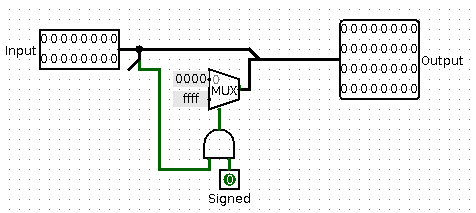
\includegraphics{Billeder/single_cycle_bit_extender.png}

\subsection{Branch control unit}
Vi har valgt at indkapsle logikken omkring valg at næste instruktion. Dette vil
formentlig også gøre det nemmere at udvidde instruktionssættet et senere
tidspunkt. Delkomponenten udfører følgende funktionalitet:

\begin{itemize}
\item Udregn næste PC i tilfælde af at der ikke branches.
\item Udregn næste PC i tilfælde af at der branches, idet der bruges en
bitforlænger på de nederste 16 bits af maskininstruktionen.\footnote{Bemærk at
bitshifting operationen vil gå godt også i de tilfælde hvor tallet er negativt.
Beviset herfor er trivielt.}
\item Beregn om der branches og brug dette resultat med en multiplexor til at
finde ud af hvilket resultat der skal bruges.
\end{itemize}

Vi har desuden valgt at implementere {\tt bne} instruktionen, idet det var
trivielt at udvidde vores control unit og branch control unit til at håndtere
dette også. Resultatet er, at der sendes 2 bits information mellem disse i
stedet for kun 1. \\
\\
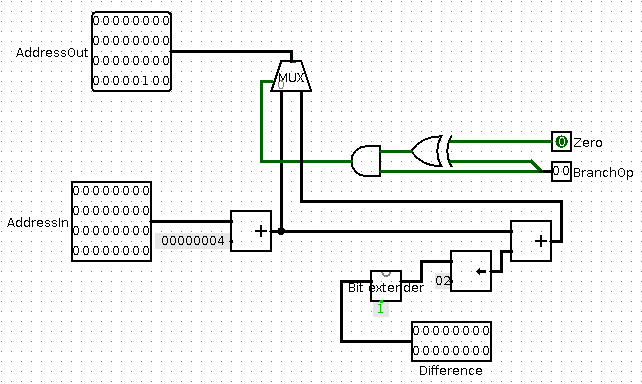
\includegraphics[angle=90]{Billeder/single_cycle_branch.png}

\subsection{ALU control unit}
Vores ALU control unit i høj grad triviel at implementere: Det er blot en
PLA. Hvad der viste sig at være et mindre problem var, at den skulle kunne
skelne mellem eksempelvis {\tt addi} og {\tt ori}. Problemet er der ud fra
specifikationen i bogen ikke er nok information til at skelne mellem disse. Vi
valgte derfor også at føre de tre bit som er forskellige mellem operationerne
ind i ALU control unit, hvorved det trivielt kunne implementeres. Desuden er der
blevet tilføjet en række i PLA'en til {\tt nor}-instruktionen, da det var
trivielt også at have den med. \\
\\
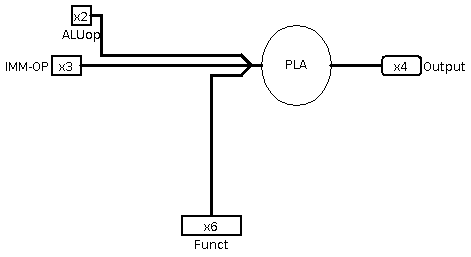
\includegraphics{Billeder/single_cycle_alucontrol.png}

\subsection{Control unit}
Vores control unit var ligesom ALU control unit i høj grad triviel men en smule
tidskrævende at implementere. Årsagen var den samme: Den eneste aktive komponent
er en PLA. Vores control unit er mere eller mindre en direkte implementation af
hvad der blev beskrevet i bogen, bortset fra følgende ændringer:

\begin{itemize}
\item Der er lavet en udgående bit til at afgøre om de nederste 16 bit af
maskininstruktionen skal fortolkes som et signed eller et unsigned tal (i de
tilfælde hvor det er relevant).
\item Branch er blevet udvidet til at indeholde 2 bits, for at implementere {\tt
bne} instruktionen.
\item Der er tilføjet yderligere rækker til de instruktioner som ikke blev
beskrevet i bogen.
\item Rækkefølgen af pins'ene er blevet ændret for at gøre det overordnede
diagram mere overskueligt.
\end{itemize}

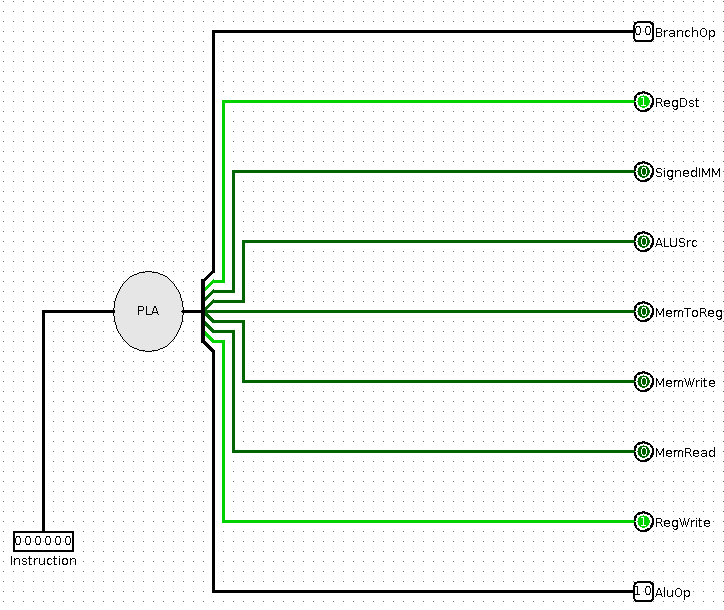
\includegraphics[angle=90,scale=0.75]{Billeder/single_cycle_control.png}

\subsection{Sammensætning}
Sammensætningen af alle delkomponenterne er også sket som i bogen, dog er der
gjort en hel del ud af at få tingene placeret så at det i vores øjne er så
overskueligt som muligt, ved eksempelvis at minimere antallet af ledninger der
krydser hinanden. Der er dog derudover følgende ændringer (som også er blevet
nævnt under de enkelte delkomponenter):

\begin{itemize}
\item Som tidligere nævnt er branch blevet udvidet til at være 2 bits for at
understøtte {\tt bne} instruktionen.
\item Bitforlængeren undersøtte både signed og unsigned værdier.
\item Logikken omkring beregning af den næste PC er flyttet til en delkomponent
for sig.
\item ALU control har nu også input pins til at kende forskel på eksempelvis
{\tt addi} og {\tt ori}.
\item Rækkefølgen af pins er flere steder blevet ændret for at gøre det
overordnede diagram mere overskueligt (dette gælder især control unit).
\item Datahukommelsesenheden bruger kun de laveste 24 bits. Desuden har den
32-bit words, som afviger fra det i bogen. Det vil sige at eksempelvis
{\tt -1(\$v0)} ikke overlapper {\tt 0(\$v0)}. Dette ville dog nemt kunne ændres,
men ville for overskuelighedens skyld nok gøres i en delkomponent.
\end{itemize}
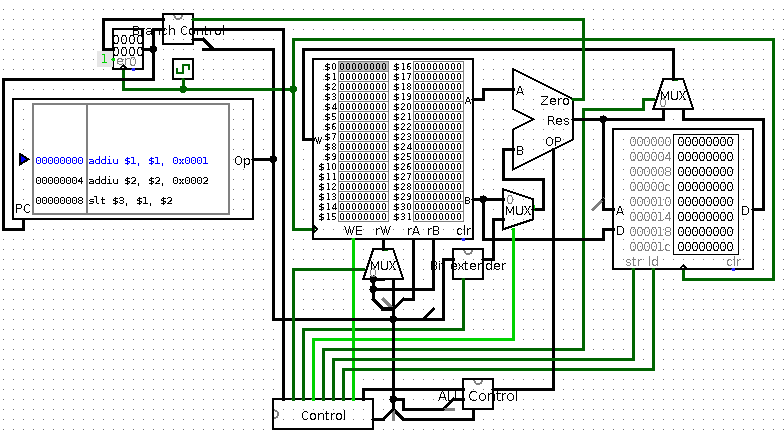
\includegraphics[angle=90,scale=0.9]{Billeder/single_cycle_main.png}
